\section{Nico Ekklesia Sembiring}
\subsection{Apa itu fungsi library matplotlib?}
Library Matplotlib berfungsi untuk membuat visualisasi yang kuat dalam menjelaskan suatu data dalam bentuk diagram dan grafik. 
Contoh grafik yang dapat digambarkan menggunakan Matplotlib adalah :
\begin{itemize}
    \item Grafik Biasa 
    \item Grafik Polar
    \item Chart
    \item Dan yang lainnya
\end{itemize}

\subsection{Jelaskan langkah-langkah membuat sumbu X dan Y di matplotlib}
Langkah langkah membuat Sumbu X dan Y adalah sebagai berikut :
\begin{itemize}
    \item Buat variabel x dan Y
    \item Masukkan nilai dari setiap variabel
    \lstinputlisting[firstline=12, lastline=13]{src/6/Teori/1174096/1174096.py}
    \item Deklarasikan nama dari sumbu x dan y 
    \lstinputlisting[firstline=16, lastline=17]{src/6/Teori/1174096/1174096.py}
\end{itemize}

Setelah dibuat, begini lah hasilnya
\begin{figure}[H]
	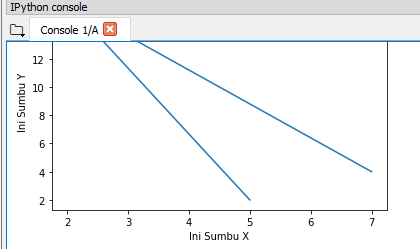
\includegraphics[width=9cm]{figures/6/Teori/1174096/1.png}
	\caption{Hasil membuat sumbu x dan y}
	\centering
\end{figure}

\subsection{Jelaskan bagaimana perbedaan fungsi dan cara pakai untuk berbagai jenis(bar,histogram,scatter,line dll) jenis plot di matplotlib}
Perbedaan fungsi dapat dilihat sebagai berikut :
\begin{itemize}
    \item Graph\linebreak
    Fungsi graph digunakan untuk membuat visualisasi berupa grafik.
    cara pakainya adalah sebagai berikut :
    \lstinputlisting[caption = fungsi untuk membuat graph., firstline=10, lastline=18]{src/6/Teori/1174096/1174096.py}
    hasilnya adalah sebagai berikut:
    \begin{figure}[H]
        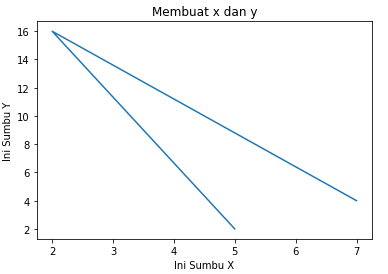
\includegraphics[width=9cm]{figures/6/Teori/1174096/3graph.png}
        \caption{Hasil graph}
        \centering
    \end{figure}

    \item Bar\linebreak 
    Fungsi Bar digunakan untuk membuat visualisasi berupa diagram batang yang berhimpit.
    Cara Pakainya adalah sebagai berikut :
    \lstinputlisting[caption = fungsi untuk membuat bar., firstline=22, lastline=32]{src/6/Teori/1174096/1174096.py}
    hasilnya adalah sebagai berikut:
    \begin{figure}[H]
        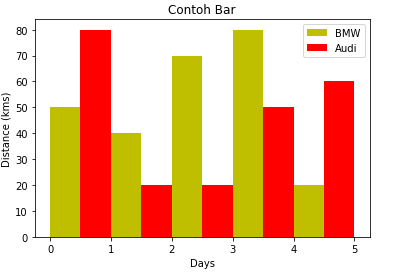
\includegraphics[width=9cm]{figures/6/Teori/1174096/3bar.png}
        \caption{Hasil bar}
        \centering
    \end{figure}

    \item Histogram\linebreak
    Fungsi Histogram digunakan untuk membuat visualisasi berupa diagram batang yang tidak berhimpit.
    Cara Pakainya adalah sebagai berikut :
    \lstinputlisting[caption = fungsi untuk membuat histogram., firstline=35, lastline=42]{src/6/Teori/1174096/1174096.py}
    hasilnya adalah sebagai berikut:
    \begin{figure}[H]
        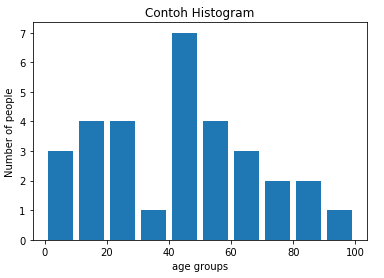
\includegraphics[width=9cm]{figures/6/Teori/1174096/3histogram.png}
        \caption{Hasil histogram}
        \centering
    \end{figure}

    \item Scatter\linebreak
    Fungsi Scatter digunakan untuk membuat visualisasi berupa titik titik.
    Cara Pakainya adalah sebagai berikut :
    \lstinputlisting[caption = fungsi untuk membuat scatter., firstline=45, lastline=58]{src/6/Teori/1174096/1174096.py}
    hasilnya adalah sebagai berikut:
    \begin{figure}[H]
        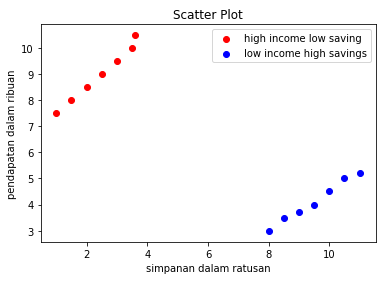
\includegraphics[width=9cm]{figures/6/Teori/1174096/3scatter.png}
        \caption{Hasil scatter}
        \centering
    \end{figure}

    \item Area plot\linebreak
    Fungsi Area plot digunakan untuk membuat visualisasi berupa area.
    Cara Pakainya adalah sebagai berikut :
    \lstinputlisting[caption = fungsi untuk membuat area plot., firstline=61, lastline=80]{src/6/Teori/1174096/1174096.py}
    hasilnya adalah sebagai berikut:
    \begin{figure}[H]
        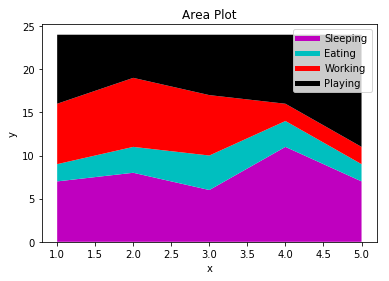
\includegraphics[width=9cm]{figures/6/Teori/1174096/3areaplot.png}
        \caption{Hasil area plot}
        \centering
    \end{figure}

    \item Pie\linebreak
    Fungsi Pie digunakan untuk membuat visualisasi berupa diagram lingkaran.
    Cara Pakainya adalah sebagai berikut :
    \lstinputlisting[caption = fungsi untuk membuat pie., firstline=83, lastline=104]{src/6/Teori/1174096/1174096.py}
    hasilnya adalah sebagai berikut:
    \begin{figure}[H]
        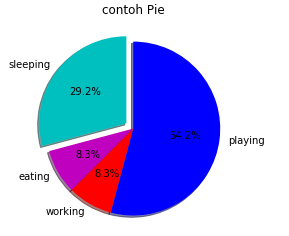
\includegraphics[width=9cm]{figures/6/Teori/1174096/3pie.png}
        \caption{Hasil pie}
        \centering
    \end{figure}
    
\end{itemize}

\subsection{Jelaskan bagaimana cara menggunakan legend dan label serta kaitannya dengan fungsi tersebut}
Fungsi legend digunakan untuk menjelaskan makna dari objek berupa titik atau garis di dalam diagram.
cara menggunakan legend adalah 
\lstinputlisting[caption = fungsi untuk membuat legend., firstline=24, lastline=28]{src/6/Teori/1174096/1174096.py}
contoh legend :
\begin{figure}[H]
    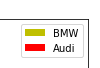
\includegraphics[width=9cm]{figures/6/Teori/1174096/4legend.png}
    \caption{contoh legend}
    \centering
\end{figure}

\subsection{Jelaskan apa fungsi dari subplot di matplotlib, dan bagaimana cara kerja dari fungsi subplot, sertakan ilustrasi dan gambar sendiri dan apa parameternya jika ingin menggambar plot dengan 9 subplot di dalamnya}
Subplot berfungsi untuk menggabungkan beberapa plot kedalam satu figure
cara kerjanya adalah sebagai berikut
\lstinputlisting[caption = cara kerja subplot., firstline=108, lastline=134]{src/6/Teori/1174096/1174096.py}
Parameter yang digunakan ketika ingin membuat 9 subplot terdiri dari (331) sampai (339). karena posisi subplot dilihat dengan melihat tinggi,lebar,urutan
hasil dari subplot adalah
\begin{figure}[H]
    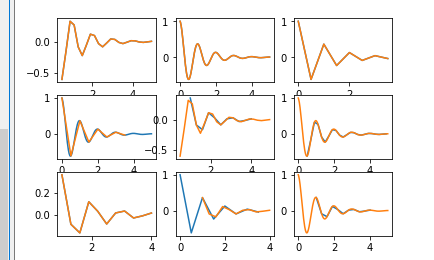
\includegraphics[width=9cm]{figures/6/Teori/1174096/5subplot.png}
    \caption{hasil subplot}
    \centering
\end{figure}

\subsection{Sebutkan semua parameter color yang bisa digunakan}
Parameter color yang bisa digunakan antara lain RGB dan CMYK
\begin{itemize}
    \item C (Cyan) adalah biru muda
    \item M (Magenta) adalah merah muda
    \item Y (Yellow) adalah kuning
    \item K (Key) adalah hitam
    \item R (Red) adalah merah
    \item G (Green) adalah Hijau
    \item B (Blue) adalah Biru
    
\end{itemize}

\subsection{Jelaskan bagaimana cara kerja dari fungsi hist, sertakan ilustrasi dan gambar sendiri}
cara kerja dari fungsi histogram adalah sebagai berikut :
\lstinputlisting[caption = cara kerja histogram., firstline=137, lastline=144]{src/6/Teori/1174096/1174096.py}
hasilnya adalah
\begin{figure}[H]
    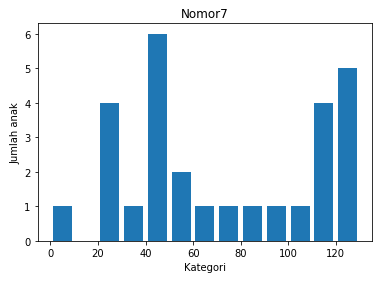
\includegraphics[width=9cm]{figures/6/Teori/1174096/7his.png}
    \caption{histogram}
    \centering
\end{figure}

\subsection{Jelaskan lebih mendalam tentang parameter dari fungsi pie diantaranya labels, colors, startangle, shadow, explode, autopct}
\begin{itemize}
    \item Labels = berfungsi untuk menampilkan tulisan pada diagram pie
    \item Colors = berfungsi untuk menentukan warna pada tiap bagian pada diagram pie
    \item Startangle = berfungsi untuk menentukan sudut pertama pada diagram pie
    \item Shadow = berfungsi untuk menampilkan efek timbul pada diagram pie
    \item Explode = berfungsi untuk menunjukkan jarak pisah dari diagram pie.
    \item Autopct = berfungsi umtuk menampilkan jumlah angka dibelakang koma pada bilangan pecahan
\end{itemize}

\subsection{Pengecekan Plagiarisme Teori}
\begin{figure}[H]
	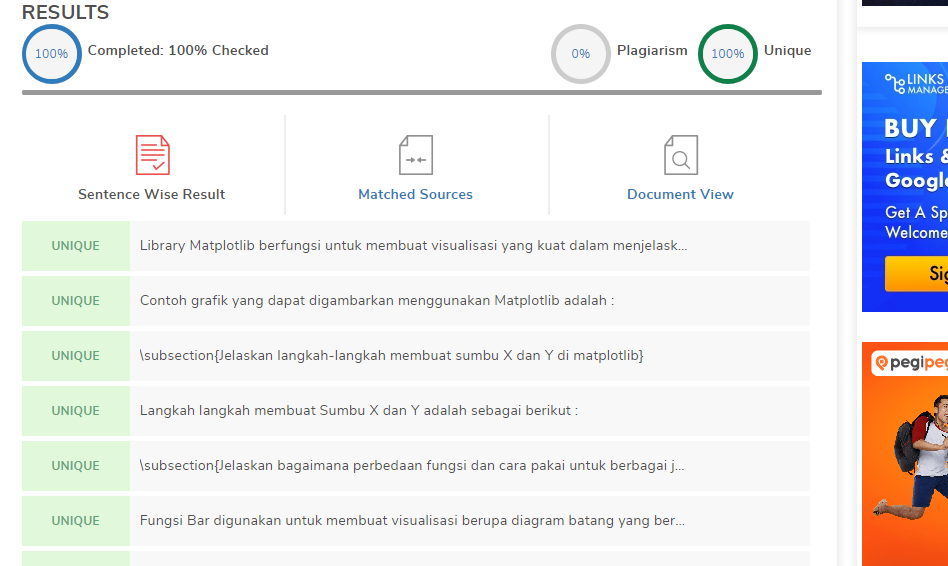
\includegraphics[width=9cm]{figures/6/Teori/1174096/Plagiat.png}
	\centering
\end{figure}

\section{Dwi Yulianingsih}
\subsection{Soal 1}
Isi jawaban soal ke-1

Kalau mau dibikin paragrap \textbf{cukup enter aja}, tidak usah pakai \verb|par| dsb

%\subsection{Soal 2}
%Isi jawaban soal ke-2

%\subsection{Soal 3}
%Isi jawaban soal ke-3

\section{Harun Ar-Rasyid}
\subsection{Soal 1}
Isi jawaban soal ke-1

Kalau mau dibikin paragrap \textbf{cukup enter aja}, tidak usah pakai \verb|par| dsb

%\subsection{Soal 2}
%Isi jawaban soal ke-2

%\subsection{Soal 3}
%Isi jawaban soal ke-3

\section{Sri Rahayu}
\subsection{Soal 1}
Isi jawaban soal ke-1

Kalau mau dibikin paragrap \textbf{cukup enter aja}, tidak usah pakai \verb|par| dsb

%\subsection{Soal 2}
%Isi jawaban soal ke-2

%\subsection{Soal 3}
%Isi jawaban soal ke-3

\section{Doli Jonviter}
\subsection{Soal 1}
Isi jawaban soal ke-1

Kalau mau dibikin paragrap \textbf{cukup enter aja}, tidak usah pakai \verb|par| dsb

%\subsection{Soal 2}
%Isi jawaban soal ke-2

%\subsection{Soal 3}
%Isi jawaban soal ke-3

\section{Rahmatul Ridha}
\subsection{Soal 1}
Isi jawaban soal ke-1

Kalau mau dibikin paragrap \textbf{cukup enter aja}, tidak usah pakai \verb|par| dsb

%\subsection{Soal 2}
%Isi jawaban soal ke-2

%\subsection{Soal 3}
%Isi jawaban soal ke-3

\section{Tomy Prawoto}
\subsection{Soal 1}
Isi jawaban soal ke-1

Kalau mau dibikin paragrap \textbf{cukup enter aja}, tidak usah pakai \verb|par| dsb

%\subsection{Soal 2}
%Isi jawaban soal ke-2

%\subsection{Soal 3}
%Isi jawaban soal ke-3
